\section{Deviations of Random Matrices on Sets}
The main question in this chapter is: How does an $m \times n$ matrix act on a general set $t \subset 
\mathbb{R}^n$? 



% ----------9.1----------
\subsection{Matrix Deviation Inequality}
Take an $m \times n$ random matrix $X$ with independent, isotropic, and subgaussian rows. The concentration of 
the norm (\cref{thm:3.1.1}) tells us that for any fixed vector $x \in \mathbb{R}^n$, the approximation 
\[ \lVert Ax \rVert_{2} \approx \sqrt{m}\lVert x \rVert_{2} \]
holds with high probability.

Let's ask something more general: Is it true that with high probability, the equation above holds 
\textit{simultaneously} for many vectors $x \in \mathbb{R}^n$? To quantify how many, pick some bounded set 
$T \subset \mathbb{R}^n$ and ask if the approximation holds simultaneously for all $x \in T$. It turns out that 
the maximal error is about $\gamma(T)$, the Gaussian complexity of $T$.

\begin{theorem}[Matrix deviation inequality]
\label{thm:9.1.1}
Let $A$ be an $m \times n$ random matrix with independent, isotropic and subgaussian rows $A_i$. Then for any 
subset $T \subset \mathbb{R}^n$, 
\[ \mathbb{E}\left[ \sup_{x \in T}\left| \lVert Ax \rVert_{2} - \sqrt{m}\lVert x \rVert_{2} \right| \right] 
\leq CK^2 \gamma(T), \]
where $\gamma(T)$ is the Gaussian complexity from Section 7.5.3, defined as 
\[ \gamma(T) = \mathbb{E}\left[ \sup_{x \in T}|\left\langle g, x \right\rangle| \right], \ g \sim N(0, I_n), \]
and $K = \max_{i} \lVert A_i \rVert_{\psi_2}$.
\end{theorem}

The plan is to deduce this from Talagrand's comparison inequality (\cref{cor:8.5.8}). To do that, we just have 
to check the random process 
\[ Z_x := \lVert Ax \rVert_{2} - \sqrt{m}\lVert x \rVert_{2} \]
indexed by vectors $x \in \mathbb{R}^n$ has subgaussian increments. Here is the claim:

\begin{theorem}[Subgaussian increments]
\label{thm:9.1.2}
Let $A$ be an $m \times n$ random matrix with independent, isotropic and subgaussian rows $A_i$. Then the random 
process $Z_x$ defined above has subgaussian increments: 
\[ \lVert Z_x - Z_y \rVert_{\psi_2} \leq CK^2 \lVert x - y \rVert_{2} \text{ for all } x, y \in \mathbb{R}^n, \]
here $K = \max_{i} \lVert A_i \rVert_{\psi_2}$.
\end{theorem}

Once we have proved this theorem, we plug it into Talagrand's comparison inequality (Exercise 8.37 (a)) and get 
\[ \mathbb{E}\left[ \sup_{x \in T} |Z_x| \right] \leq CK^2 \gamma(T) \]
which directly gives \cref{thm:9.1.1}. So, all we have to do is prove \cref{thm:9.1.2} - and it is in fact 
easier since it's for fixed $x$ and $y$.

\begin{proof}[Proof of \cref{thm:9.1.2}]
This argument will be a bit longer than usual, so we'll (hopefully) make it easier by starting with simpler 
cases and building up from there.

\textbf{Step 1: Unit vector $x$ and zero vector $y$.} If $\lVert x \rVert_{2} = 1$ and $y = 0$, the inequality 
in the theorem statement becomes 
\[ \left\lVert \lVert Ax \rVert_{2} - \sqrt{m} \right\rVert_{\psi_2} \leq CK^2. \]
The random vector $Ax \in \mathbb{R}^m$ has independent, subgaussian coordinates $\left\langle A_i, x
\right\rangle$, which satisfy 
\[ \mathbb{E}\left[ \left\langle A_i, x \right\rangle^2 \right] = 1 \] 
by isotropy. So, the equation above follows from the concentration of the norm (\cref{thm:3.1.1}).

\textbf{Step 2: Unit vectors $x, y$ and the squared process.} Assume now that 
\[ \lVert x \rVert_{2} = \lVert y \rVert_{2} = 1. \]
In this case, the inequality in the theorem statement becomes 
\[ \left\lVert \lVert Ax \rVert_{2} - \lVert Ay \rVert_{2} \right\rVert_{\psi_2} \leq 
CK^2 \lVert x - y \rVert_{2}. \quad (*) \]
Since the \textit{squared} $\ell^2$ norm would be simpler to work with (no square roots), let's prove a version 
of the equation above with squared norms. Here's a good guess to what it should look like: with high probability,
\begin{align*}
	\lVert Ax \rVert_{2}^2 - \lVert Ay \rVert_{2}^2 
	&= (\lVert Ax \rVert_{2} + \lVert Ay \rVert_{2}) \cdot (\lVert Ax \rVert_{2} - \lVert Ay \rVert_{2}) \\
	&\lesssim \sqrt{m} \cdot \lVert x - y \rVert_{2}.
\end{align*}
This seems reasonable because $\lVert Ax \rVert_{2}$ and $\lVert Ay \rVert_{2}$ are roughly $\sqrt{m}$ by step 
1, and hence we expect $(*)$ to hold.

Let's go ahead and prove this. Expand the matrix-vector product:
\[ \lVert Ax \rVert_{2}^2 - \lVert Ay \rVert_{2}^2 
= \sum_{i = 1}^{m} (\left\langle A_i, x \right\rangle^2 - \left\langle A_i, y \right\rangle^2) 
= \sum_{i = 1}^{m} \left\langle A_i, x + y \right\rangle \left\langle A_i, x - y \right\rangle, \]
then dividing both sides by $\lVert x - y \rVert_{2}$, getting 
\[ \Delta := \frac{\lVert Ax \rVert_{2}^2 - \lVert Ay \rVert_{2}^2}{\lVert x - y \rVert_{2}^2} 
= \sum_{i = 1}^{m} \left\langle A_i, u \right\rangle \left\langle A_i, v \right\rangle, \]
where 
\[ u := x + y \text{ and } v := \frac{x - y}{\lVert x - y \rVert_{2}}. \]
Our goal is to show that $|\Delta| \lesssim \sqrt{m}$ with high probability.

What do we see in $\Delta$? A sum of \textit{independent} random variables $\left\langle A_i, u \right\rangle 
\left\langle A_i, v \right\rangle$! They are mean-zero, because by construction we have 
\[ \left\langle A_i, u \right\rangle \left\langle A_i, v \right\rangle = 
\frac{\left\langle A_i, x \right\rangle^2 - \left\langle A_i, y \right\rangle^2}{\lVert x - y \rVert_{2}}, \]
and by isotropy, 
\[ \mathbb{E}\left[ \left\langle A_i, x \right\rangle^2 - \left\langle A_i, y \right\rangle^2 \right] 
= 1 - 1 = 0. \]
Moreover, these are \textit{subexponential}. \cref{lem:2.8.6} and the subgaussian assumption on $A_i$ give 
\begin{align*}
	\lVert \left\langle A_i, u \right\rangle \left\langle A_i, v \right\rangle \rVert_{\psi_1} 
	&\leq \lVert \left\langle A_i, u \right\rangle \rVert_{\psi_2} \cdot 
	\lVert \left\langle A_i, v \right\rangle \rVert_{\psi_2} \\
	&\leq K \lVert u \rVert_{2} \cdot K \lVert v \rVert_{2} \\
	&\leq 2K^2
\end{align*}
where in the last step, we used that $\lVert u \rVert_{2} \leq \lVert x \rVert_{2} + \lVert y \rVert_{2} \leq 2$ 
and $\lVert v \rVert_{2} = 1$. So we can apply Bernstein's inequality (\cref{thm:2.9.1}) and get 
\[ P(|\Delta| \geq t \sqrt{m}) \leq 2 \exp{\left[ -c \min_{}\left( \frac{t^2}{K^4}, \frac{t \sqrt{m}}{K^2} 
\right) \right]} \leq 2 \exp{\left( -\frac{c_1 t^2}{K^4} \right)} \]
for any $0 \leq t \leq \sqrt{m}$.

\textbf{Step 3: Unit vector $x, y$ and the original process.} Now let's get rid of the squares and prove the 
original inequality $(*)$ for all unit vectors $x$ and $y$.

Using the definition of the subgaussian norm (\cref{prop:2.6.6} (i) and \cref{rmk:2.6.3}), $(*)$ becomes 
\[ p(s) := P \left( \frac{|\lVert Ax \rVert_{2} - \lVert Ay \rVert_{2}|}{\lVert x - y \rVert_{2}^2} \right) 
\leq 4 \exp{\left( -\frac{cs^2}{K^2} \right)} \text{ for all } s > 0. \]
(Here the constant 4 instead of 2 will give us a little more room to maneuver.)

Now we have two cases:
\textit{Case 1:} $s \leq 2 \sqrt{m}$. Let's use the result from step 2. To use it, multiply both sides of the 
inequality that defines $p(s)$ by $\lVert Ax \rVert_{2} + \lVert Ay \rVert_{2}$, and recall the definition of 
$\Delta$ to get 
\[ p(s) = P(|\Delta| \geq s(\lVert Ax \rVert_{2} + \lVert Ay \rVert_{2})) 
\leq P(|\Delta| \geq s \lVert Ax \rVert_{2}). \]
We know from step 2 that $\lVert Ax \rVert_{2} \approx \sqrt{m}$ with high probability. So it makes sense to 
consider two cases: THe likely case where $\lVert Ax \rVert_{2} \geq \sqrt{m}/2$ and thus $|\Delta| \geq 
s \sqrt{m}/2$, and the unlikely case where $\lVert Ax \rVert_{2} < \sqrt{m}/2$ (and we deop the clause about 
$\Delta$, only increasing the probability). This leads to 
\[ p(s) \leq P \left( |\Delta| \geq \frac{s \sqrt{m}}{2} \right) + P \left( \lVert Ax \rVert_{2} 
< \frac{\sqrt{m}}{2} \right) = p_1(s) + p_2(s). \]
The result from Step 2 handles the likely case:
\[ p_1(s) \leq 2 \exp{\left( -\frac{cs^2}{K^4} \right)}, \]
while the result of Step 1 together with the triangle inequality handle the unlikely case: 
\[ p_2(s) \leq P \left( |\lVert Ax \rVert_{2} - \sqrt{m}| > \frac{\sqrt{m}}{2} \right) 
\leq 2 \exp{\left( -\frac{cs^2}{K^4} \right)}.\]
Adding up the two, we get the desired bound:
\[ p(s) \leq 4 \exp{\left( -\frac{cs^2}{K^4} \right)}. \]

\textit{Case 2:} $s > 2 \sqrt{m}$. By the triangle inequality, $|\lVert Ax \rVert_{2} - \lVert Ay \rVert_{2}| 
\leq \lVert A(x - y) \rVert_{2}$, so 
\begin{align*}
	p(s) \leq P(\lVert Au \rVert_{2} \geq s) \quad (u = \frac{x - y}{\lVert x - y \rVert_{2}} 
	\text{ as before}) \\
	&\leq P(\lVert Au \rVert_{2} - \sqrt{m} \geq s/2) \quad (\text{Since } s > 2 \sqrt{m}) \\
	&\leq 2 \exp{\left( -\frac{cs^2}{K^4} \right)} \quad \text{(By step 1)}.
\end{align*}
Therefore in either case, we get the desired bound.

\textbf{Step 4: Full generality.} Finally, let's show the result for arbitrary $x, y \in \mathbb{R}^n$. By 
scaling, we can assume without loss of generality that 
\[ \lVert x \rVert_{2} = 1 \text{ and } \lVert y \rVert_{2} \geq 1. \]
Project $Y$ onto the unit sphere, i.e. consider $\bar{y} := y / \lVert y \rVert_{2}$ (See figure 9.1):
\begin{center}
	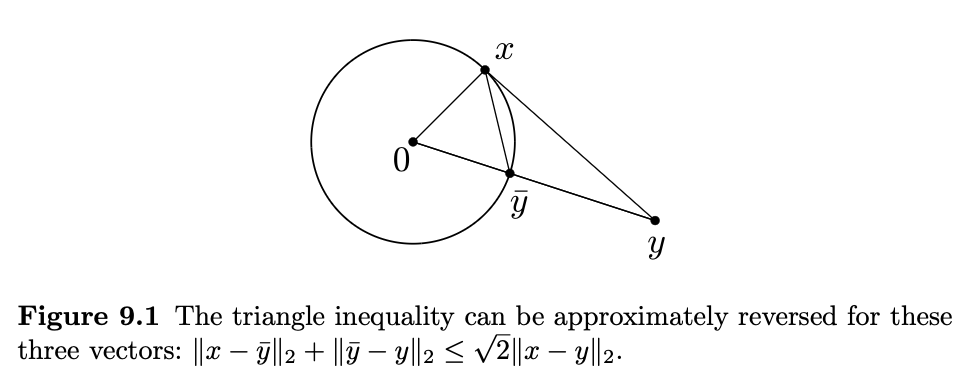
\includegraphics[width=0.8\textwidth]{Chapter 9/fig9-1.png}
\end{center}
Then by triangle inequality:
\[ \lVert Z_x - Z_y \rVert_{\psi_2} \leq \lVert Z_x - Z_{\bar{y}} \rVert_{\psi_2} 
+ \lVert Z_{\bar{y}} - Z_y \rVert_{\psi_2}. \]
Since both $x, \bar{y}$ are unit vectors, the result of Step 3 handles the first term:
\[ \lVert Z_x - Z_{\bar{y}} \rVert_{\psi_2} \leq CK^2 \lVert x - \bar{y} \rVert_{2}. \]
To handle the second term, note that $\bar{y}$ and $y$ are colinear vectors. So by homogeneity, 
\[ \lVert Z_{\bar{y}} - Z_y \rVert_{\psi_2} = \lVert \bar{y} - y \rVert_{2} \cdot \lVert Z_{\bar{y}} 
\rVert_{\psi_2}. \]
Now, since $\bar{y}$ is a unit vector, the result of Step 1 gives $\lVert Z_{\bar{y}} \rVert_{\psi_2} 
\leq CK^2$. Conbining the two terms, we conclude that 
\[ \lVert Z_x - Z_y \rVert_{\psi_2} \leq CK^2 (\lVert x - \bar{y} \rVert_{2} + \lVert \bar{y} - y \rVert_{2}). \]
At first this looks bad - we wnat to bound right hand side by $\lVert x - y \rVert_{2}$, but the triangle 
inequality goes the other way! Luckily, in our case (via the projection of $y$), the triangle inequality can be 
approximately reversed (Exercise 9.1):
\[ \lVert x - \bar{y} \rVert_{2} + \lVert \bar{y} - y \rVert_{2} \leq \sqrt{2}\lVert x - y \rVert_{2}. \]
Plugging this into the bound above, we get the desired bound:
\[ \lVert Z_x - Z_y \rVert_{\psi_2} \leq \sqrt{2}CK^2 \lVert x - y \rVert_{2}, \]
which proves the theorem.
\end{proof}

\begin{remark}[Matrix deviations from the mean]
\label{rmk:9.1.3}
A quick centering trick turns \cref{thm:9.1.1} into a deviation inequality around the mean 
$\mathbb{E}\left[ \lVert Ax \rVert_{2} \right]$ (Exercise 9.2).
\end{remark}

\begin{remark}[Matrix deviations: a high-probability bound]
\label{rmk:9.1.4}
We only stated \cref{thm:9.1.1} as an expectation bound, but we can upgrade it to a high-probability bound via 
the high-probability version of Talagrand's inequality (Exercise 8.37(b)). For any $u \geq 0$, the event 
\[ \sup_{x \in T} \left| \lVert Ax \rVert_{2} - \sqrt{m}\lVert x \rVert_{2} \right| 
\leq CK^2 [w(T) + u \cdot \mathrm{rad}(T)] \]
holds with probability at least $1 - 2 \exp{(-u^2)}$. Can you see why the above implies the expectation bound?
\end{remark}

\begin{remark}[Matrix deviations of squares]
\label{rmk:9.1.5}
If you are interested in deviations of the quadratic process $\lVert Ax \rVert_{2}^2$, we can also deduce this 
from \cref{thm:9.1.1} (Exercise 9.3):
\[ \mathbb{E}\left[ \sup_{x \in T} \left| \lVert Ax \rVert_{2}^2 - m \lVert x \rVert_{2}^2 \right| \right] 
\leq CK^4 \gamma(T)^2 + CK^2 \sqrt{m} \mathrm{rad}(T) \gamma(T). \]
\end{remark}



% ----------9.2----------
\subsection{Random Matrices, Covariance Estimation, and Johnson-Lindenstrauss}
The matrix deviation inequality has lots of useful consequences. We'll go over a few of them in this chapter!


\subsubsection{Singular Values of Random Matrices}
Applying the matrix deviation inequality for the unit Euclidean sphere $T = S^{n - 1}$ gives us the singular 
value bounds from Chapter 4.

Here is the quick check: since for the sphere we have 
\[ \mathrm{rad}(T) = 1 \text{ and } w(T) \leq \sqrt{n}, \]
the matrix deviation inequality shows that the event 
\[ \sqrt{m} - CK^2 (\sqrt{n} + u) \leq \lVert Ax \rVert_{2} \leq \sqrt{m} + CK^2 (\sqrt{n} + u) \text{ for 
all } x \in S^{n - 1} \]
holds with probability at least $1 - 2 \exp{(-u^2)}$. Then taking the min/max gives 
\[ \sqrt{m} - CK^2 (\sqrt{n} + u) \leq \sigma_n(A) \leq \sigma_1(A) \leq \sqrt{m} + CK^2 (\sqrt{n} + u) 
\text{ for all } x \in S^{n - 1}, \]
giving \cref{thm:4.6.1} in a different way.


\subsubsection{Random Projections of Sets}
From the matrix deviation inequality, we also get a sharper bound on the random projection bound in Section 7.6:

\begin{proposition}[Sizes of random projections of sets]
\label{prop:9.2.1}
Let $T \subset \mathbb{R}^n$ be a bounded set, and let $A$ be an $m \times n$ matrix with independent, isotropic 
and subgaussian rows $A_i$. Then the scaled matrix $P = \frac{1}{\sqrt{n}}A$ (a subgaussian projection) satisfies
\[ \mathbb{E}\left[ \mathrm{diam}(PT) \right] \leq \sqrt{\frac{m}{n}}\mathrm{diam}(T) + CK^2 w_s(T). \]
Here $K = \max_{i}\lVert A_i \rVert_{\psi_2}$ and $w_s(T)$ is the spherical width of $T$.
\end{proposition}

\begin{proof}
\cref{thm:9.1.1} implies via triangle inequality:
\[ \mathbb{E}\left[ \sup_{x \in T}\lVert Ax \rVert_{2} \right] \leq \sqrt{m}\sup_{x \in T}\lVert x \rVert_{2} 
+ CK^2 \gamma(T), \]
which we can rewrite in terms of the radii of $AT$ and $T$:
\[ \mathbb{E}\left[ \mathrm{rad}(AT) \right] \leq \sqrt{m}\mathrm{rad}(T) + CK^2 \gamma(T). \]
Applying this bound for the difference set $T - T$ instead of $T$ to get 
\[ \mathbb{E}\left[ \mathrm{diam}(AT) \right] \leq \sqrt{m}\mathrm{diam}(T) + 2CK^2w(T), \]
where we used \cref{lem:7.5.11} (a) to pass from Gaussian complexity to Gaussian width. Divide both sides by 
$\sqrt{n}$ completes the proof.
\end{proof}


\subsubsection{Covariance Estimation for Low-dimensional Distributions}



\subsubsection{Johnson-Lindenstrauss Lemma for Infinite Sets}
The matrix deviation inequality quickly recovers the Johnson-Lindenstrauss lemma from Section 5.3 - and extends 
it to general, possibly infinite, sets.

To get a version of the JL lemma from matrix deviation, fix any $N$-point set $\mathcal{X} \in \mathbb{R}^n$ 
and consider the normalized differences: 
\[ T := \left\{ \frac{x - y}{\lVert x - y \rVert_{2}}: \ x, y \in \mathcal{X} \text{ distinct} \right\}. \]
The Gaussian complexity of $T$ satisfies 
\[ \gamma(T) \leq C \sqrt{\log_{}{N}}. \]
The matrix deviation inequality (\cref{thm:9.1.1}) shows that with high probability, 
\[ \sup_{x, y \in \mathcal{X}} \left| \frac{\lVert Ax - Ay \rVert_{2}}{\lVert x - y \rVert_{2}} - 
\sqrt{m} \right| \lesssim \sqrt{\log_{}{N}}. \]
Rearranging the terms, rewrite this as follows: the random matrix $Q := \frac{1}{\sqrt{m}}A$ is an approximate 
isometry on $\mathcal{X}$, i.e.
\[ (1 - \varepsilon)\lVert x - y \rVert_{2} \leq \lVert Qx - Qy \rVert_{2} \leq (1 + \varepsilon)\lVert x - y
\rVert_{2} \text{ for all } x, y \in \mathcal{X}, \]
for some $\varepsilon \asymp \sqrt{\log_{}{(N)} / m}$. Equivalently, if we fix $\varepsilon > 0$ and choose 
\[ m \gtrsim \varepsilon^{-2} \log_{}{N}, \]
then with high probability $Q$ is an $\varepsilon$-isometry on $\mathcal{X}$, which recovers a version of the 
classical JL lemma.

What we just not gave did not care if $\mathcal{X}$ is finite or not - all that matters is the Gaussian width. 
So we can extend JL to any set:




% ----------9.3----------
\subsection{Random Sections: The \texorpdfstring{$M^*$}{} Bound and Escape Theorem}
Here is a surprising high-dimensional fact: if you slice a convex set $T \subset \mathbb{R}^n$ with a random 
subspace $E$ of codimension $m$, the slice $T \subset E$ is often tiny - even when $m \ll n$ and $E$ is near 
full-dimensional! Let's see how this follows from the matrix deviation inequality.


\subsubsection{The \texorpdfstring{$M^*$}{} Bound}
It is handy to model a random subspace $E$ as the kernel of an $m \times n$ random matrix: $E = \ker{A}$. We 
always have 
\[ \dim{(E)} \geq n - m, \]
and if $A$ has a continuous distribution, $\dim{(E)} \geq n - m$ almost surely.

A great example is a Gaussian matrix $A$ with i.i.d. $N(0, 1)$ entries - by rotation invariance, $E - \ker{(A)}$ 
is uniformly distributed in the Grassmanian:
\[ E \sim \mathrm{Unif}(G_{n, n - m}). \]

\begin{theorem}[$M^*$ bound]
\label{thm:9.3.1}
Let $T \subset \mathbb{R}^n$ be a bounded set, and $A$ be an $m \times n$ random matrix with independent, 
isotropic and subgaussian rows $A_i$. Then the random subspace $E = \ker{A}$ satisfies 
\[ \mathbb{E}\left[ \mathrm{diam}(T \cap E) \right] \leq \frac{CK^2 w(T)}{\sqrt{m}}, \]
where $K = \max_{i}\lVert A_i \rVert_{\psi_2}$.
\end{theorem}

\begin{proof}
Apply \cref{thm:9.1.1} for $T - T$:
\[ \mathbb{E}\left[ \sup_{x, y \in T} \left| \lVert Ax - Ay \rVert_{2} - \sqrt{m}\lVert x - y \rVert_{2} \right| 
\leq CK^2 \gamma(T - T) = 2CK^2 w(T), \right] \]
by \cref{lem:7.5.11} (a). Considering only the points $x, y$ in the kernel of $A$ makes $\lVert Ax - Ay 
\rVert_{2}$ disappear since $Ax = Ay = 0$. Divide both sides by $\sqrt{m}$ to get 
\[ \mathbb{E}\left[ \sup_{x, y \in T \cap \ker{A}} \lVert x - y \rVert_{2} \right] 
\leq \frac{CK^2 w(T)}{\sqrt{m}}, \]
which is exactly what we claimed.
\end{proof}

\begin{example}[The cross-polytope]
Let's apply the $M^*$ bound to the cross-polytope $B_1^n$ - the unit ball of the $\ell^1$ norm. Since its 
Gaussian width id roughly $\sqrt{\log_{}{n}}$ by \cref{ex:7.5.8}, we get 
\[ \mathbb{E}\left[ \mathrm{diam}(B_1^n \cap E) \right] \lesssim \sqrt{\frac{\log_{}{n}}{m}}. \]
For example, if $m = 0.01n$, then 
\[ \mathbb{E}\left[ \mathrm{diam}(T \cap E) \right] \lesssim \sqrt{\frac{\log_{}{n}}{n}}. \]
So, a random $0.99n$-dimensional slice of a cross-polytope is tiny!
\end{example}

How can this be? This relates to what we discussed in \cref{rmk:7.5.10}. The ``bulk" of $B_1^n$ is concentrated 
near the inscribed ball of radius $1/\sqrt{n}$, while the rest stretches out into long, thin ``spikes" along 
the coordinate axes. A random subspace $E$ probably misses those spikes and cuts through the bulk (Figure 9.2a). 
Therefore the slice ends up with diameter about $O(1/\sqrt{n})$, maybe with a log factor as shown above. This 
intuition can be extended to general convex sets as well.

\begin{center}
	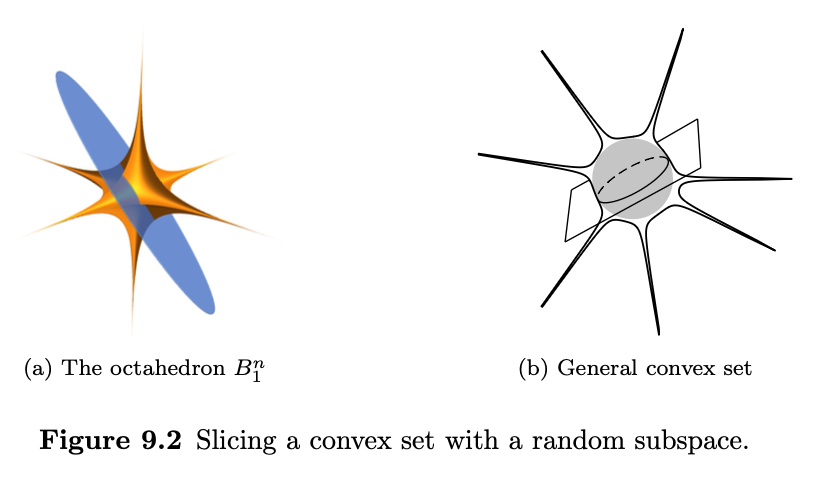
\includegraphics[width=0.8\textwidth]{Chapter 9/fig9-2.png}
\end{center}

\begin{remark}[Effective dimension]
\label{rmk:9.3.3}
To get more intuition, write the $M^*$ bound using the effective dimension (\cref{def:7.5.12}). The $M^*$ bound 
shows that slicing shrinks the dimaeter:
\[ \mathbb{E}\left[ \mathrm{diam}(T \cap E) \right] \leq 0.01 \cdot \mathrm{diam}(T) \]
as long as $m \gtrsim d(T)$. Since $\dim{(E)} = n - m$, this condition is equivalent to 
\[ \dim{(E)} + cd(T) \leq n. \]
That lines up with the linear algebra intuition: If $T$ is a cnetered Euclidean ball in some subspace 
$F \subset \mathbb{R}^n$, slicing can shrink the diameter of $T$ only when $\dim{E} + \dim{F} \leq n$.
\end{remark}


\subsubsection{The Escape Theorem}
When does a random subspace $E$ miss a given set $T$ entirely with high probability? Not if $T$ contains the 
origin - but if $T$ lies on the unit sphere (Figure 9.3), then it does as long as the codimension of $E$ is not 
too small: 

\begin{center}
	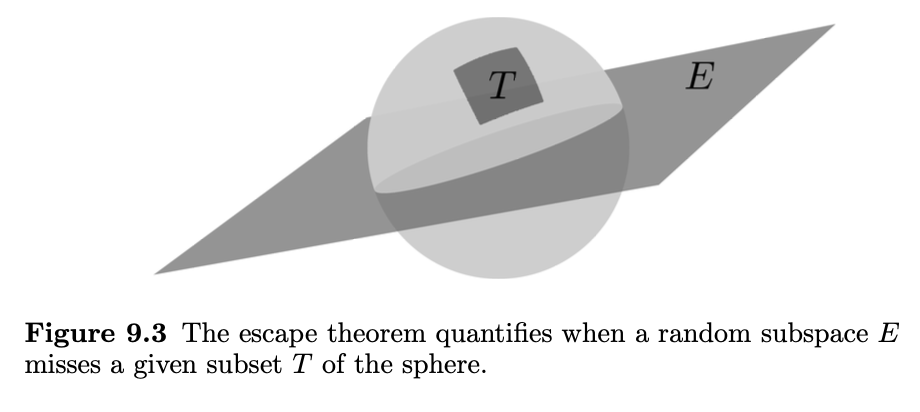
\includegraphics[width=0.8\textwidth]{Chapter 9/fig9-3.png}
\end{center}

\begin{theorem}[Escape theorem]
\label{thm:9.3.4}
Let $T \subset S^{n - 1}$ be any set, and let $A$ be an $m \times n$ matrix with independent, isotropic and 
subgaussian rows $A_i$. If 
\[ m \geq CK^4 w(T)^2, \]
then the random subspace $E = \ker{A}$ satisfies 
\[ T \cap E = \emptyset \]
with probability ar least $1 - 2 \exp{(-cm/K^4)}$. Here $K = \max_{i}\lVert A_i \rVert_{\psi_2}$.
\end{theorem}

\begin{proof}
Let us use the high-probability version of the matrix deviation inequality (\cref{rmk:9.1.4}): With probability 
at least $1 - 2 \exp{(-u^2)}$, 
\[ \sup_{x \in T}\left| \lVert Ax \rVert_{2} - \sqrt{m} \right| \leq C_1K^2(w(T) + u). \]
Suppose the above occurs. If $T \cap E \neq \emptyset$, then for any $x \in T \cap E$ we have $Ax = 0$, so 
\[ \sqrt{m} \leq C_1 K^2 (w(T) + u). \]
Set $u = \sqrt{m}/(2C_1K^2)$ and simplify this bound to get 
\[ \sqrt{m} \leq 2 C_1 K^2 w(T), \]
which contradicts the assumption if $C$ is large enough.Therefore, with that choice of $u$, the event implies 
$T \cap E = \emptyset$. Done!
\end{proof}


% ----------9.4----------
\subsection{Application: High-dimensional Linear Models}



% ----------9.5----------
\subsection{Application: Exact Sparse Recovery}



% ----------9.6----------
\subsection{Deviations of Random Matrices for General Norms}
We can generalize the matrix deviation inequality (\cref{thm:9.1.1}) to work for any norm - not just the 
Euclidean one. Actually we don't even need the noem to be nonnegative - just homogeneity and triangle inequality 
is enough.

\begin{definition}[]
\label{def:9.6.1}
A real-valued function $f$ on a linear vector space $V$ is called:
\begin{itemize}
	\item \underline{Positive-homogeneous} if $f(\alpha x) = \alpha f(x)$ for all $\alpha \geq 0$ and $x \in V$;
	\item \underline{Subadditive} if $f(x + y) \leq f(x) + f(y)$ for all $x, y \in V$.
\end{itemize}
\end{definition}

\begin{example}[]
\label{ex:9.6.2}
These functions are positive-homogeneous and subadditive:
\begin{enumerate}
	\item Any norm;
	\item Any real-valued linear function (i.e. any \textit{linear functional});
	\item In particular, the function $f(x) = x^T y$ for any fixed vector $y \in \mathbb{R}^m$;
	\item the \textit{support function} of any bounded set $S \subset \mathbb{R}^n$, defined by 
	\[ f(x) := \sup_{y \in S}\left\langle x, y \right\rangle, \ x \in \mathbb{R}^m. \]
\end{enumerate}
\end{example}

We can make \cref{thm:9.1.1} work for all norms (even positive-homogeneous, subadditive functions), but with a 
tradeoff - it applies only to Gaussian matrices:

\begin{theorem}[General matrix deviation inequality]
\label{thm:9.6.3}
Let $A$ be an $m \times n$ random matrix with i.i.d. $N(0, 1)$ entries. Let $f: \mathbb{R}^m \to \mathbb{R}$ be 
a bounded, positive-homogeneous and subadditive function, and let $b \in \mathbb{R}$ such that 
\[ f(x) \leq b \lVert x \rVert_{2} \text{ for all } x \in \mathbb{R}^n. \]
Then for any subset $T \subset \mathbb{R}^n$, 
\[ \mathbb{E}\left[ \sup_{x \in T} \left| f(Ax) - \mathbb{E}\left[ f(Ax) \right] \right| \right] 
\leq Cb \gamma(T), \]
where $\gamma(T)$ is the Gaussian complexity.
\end{theorem}

With the same logic as in the proof for \cref{thm:9.1.1}, \cref{thm:9.6.3} would immediately follow from 
Talagrand's comparison inequality once we show that the random process
\[ Z_x := f(Ax) - \mathbb{E}\left[ f(Ax) \right] \]
has subgaussian increments. Let's do this :)

\begin{theorem}[Subgaussian increments]
\label{thm:9.6.4}
Let $A$ be an $m \times n$ Gaussian random matrix with i.i.d. $N(0, 1)$ entries, and let $f: \mathbb{R}^m \to 
\mathbb{R}$ be a positive homogeneous and subadditive function satisfying 
\[ f(x) \leq b \lVert x \rVert_{2} \text{ for all } x \in \mathbb{R}^n. \]
Then the random process 
\[ Z_x := f(Ax) - \mathbb{E}\left[ f(Ax) \right] \]
has subgaussian increments:
\[ \lVert Z_x - Z_y \rVert_{\psi_2} \leq Cb \lVert x - y \rVert_{2} \text{ for all } x, y \in \mathbb{R}^n. \]
\end{theorem}

\begin{proof}
Without loss of generality, we may assume that $b = 1$. Just like in the proof of \cref{thm:9.1.2}, first assume 
that 
\[ \lVert x \rVert_{2} = \lVert y \rVert_{2} = 1. \]
In this case, the inequality in the theorem becomes 
\[ \lVert f(Ax) - f(Ay) \rVert_{\psi_2} \leq C \lVert x - y \rVert_{2}. \]

\textbf{Step 1: Creating independence.} Consider the vectors 
\[ u := \frac{x + y}{2}, \ v := \frac{x - y}{2}. \]
Then $x = u + v$ and $y = u - v$, and thus 
\[ Ax = Au + Av, \ Ay = Au - Av \quad (\text{See Figure 9.8 below}) \]
\begin{center}
	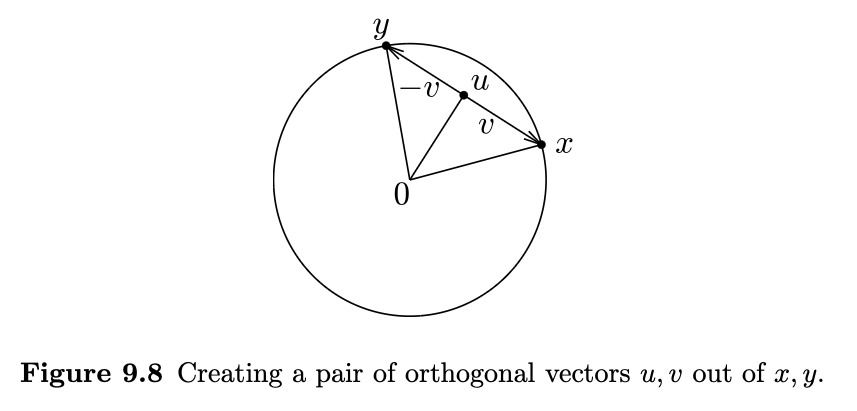
\includegraphics[width=0.8\textwidth]{Chapter 9/fig9-8.png}
\end{center}
Since $u, v$ are orthogonal, the Gaussian random vectors $Au$ and $Av$ are independent (Exercise 3.20).

\textbf{Step 2: Using Gaussian concentration.} Let's condition on $a := Au$ and study the conditional 
distribution of 
\[ f(Ax) = f(a + Av). \]
By independence, $a + Av$ is a Gaussian random vector that we can write as 
\[ a + Av = a + \lVert v \rVert_{2}g, \text{ where } g \sim N(0, I_m) \quad (\text{Exercise 3.20}) \]
We claim that the function 
\[ z \mapsto f(a + \lVert v \rVert_{2}z) \]
is Lipschitz with respect to the Euclidean norm on $\mathbb{R}^m$, with Lipschitz norm bounded by $\lVert v
\rVert_{2}$. To check this, fix any $t, s \in \mathbb{R}^m$ and use subadditivity of $f$ (in the form of 
Exercise 9.34) to get 
\begin{align*}
	f(a + \lVert v \rVert_{2}t) - f(a + \lVert v \rVert_{2}s) 
	&\leq f(\lVert v \rVert_{2}t - \lVert v \rVert_{2}s) \\
	&= \lVert v \rVert_{2} f(t - s) \quad \text{(Positive homogeneity)} \\
	&\leq \lVert v \rVert_{2} \lVert t - s \rVert_{2} \quad (b = 1),
\end{align*}
proving the claim.

Concentration in the Gauss space (\cref{thm:5.2.3}) then yields 
\[ \lVert f(a + Av) - \mathbb{E}_a\left[ f(a + Av) \right] \rVert_{\psi_2(a)}2 \leq C \lVert v \rVert_{2}, \]
where the index ``a" reminds us that these bounds are valid for the conditional distribution with $a = Au$ fixed.

\textbf{Step 3: Removing the conditioning.} Since the random vector $a - Av$ has the same distribution as that 
of $a + Av$, it satisfies the same bound:
\[ \lVert f(a - Av) - \mathbb{E}_a\left[ f(a - Av) \right] \rVert_{\psi_2(a)} \leq C \lVert v \rVert_{2}, \]
Subtract the bottom equation from the top one, use the triangle inequality and the fact that the expectations 
are the same gives 
\[ \lVert f(a + Av) - f(a - Av) \rVert_{\psi_2(a)} \leq 2 C \lVert v \rVert_{2}. \]
This bound holds conditionally for any fixed $a = Au$, Therefore, it holds for the original distribution too:
\[ \lVert f(a + Av) - f(a - Av) \rVert_{\psi_2} \leq 2 C \lVert v \rVert_{2}. \]
Passing back the the $x, y$ notation, we obtained the desired inequality.

We proved the theorem for unit vectors $x, y$. To extend it to the general case, argue exactly as step 4 in the 
proof of \cref{thm:9.1.2}.
\end{proof}

\begin{remark}[]
\label{rmk:9.6.5}
It is an open question if \cref{thm:9.6.3} holds for general subgaussian matrices $A$.
\end{remark}



% ----------9.7----------
\subsection{Two-sided Chevet Inequality and Dvoretzky-Milman Theorem}


\subsubsection{Two-sided Chevet's Inequality}
Another consequence of general matrix deviation is a sharper version of Chevet's inequality:

\begin{theorem}[Two-sided Chevet's inequality]
\label{thm:9.7.1}
Let $A$ be an $m \times n$ Gaussian random matrix with i.i.d $N(0, 1)$ entries. Let $T \subset \mathbb{R}^n$ and 
$S \subset \mathbb{R}^m$ be arbitrary bounded sets. Then 
\[ \mathbb{E}\left[ \sup_{x \in T} \left| \sup_{y \in S}\left\langle Ax, y \right\rangle - w(S) \lVert x 
\rVert_{2} \right| \right] \leq C \gamma(T) \mathrm{rad}(S), \]
where $\gamma(T)$ is the Gaussian complexity and $\mathrm{rad}(T)$ is the radius.
\end{theorem}

\begin{proof}
Let's apply \cref{thm:9.6.3} for the support function of $S$:
\[ f(x) = \sup_{y \in S}\left\langle x, y \right\rangle. \]
This is a bounded function, since the Cauchy-Schwartz inequality gives 
\[ f(x) \leq \sup_{y \in S}\lVert x \rVert_{2}\lVert y \rVert_{2} = \mathrm{rad}(S) \lVert x \rVert_{2} 
\text{ for all } x \in \mathbb{R}^n. \quad (*) \]
Since $Ax$ has the same distribution as $g \lVert x \rVert_{2}$ where $g \sim N(0, I_m)$ from Exercise 3.20, 
we have that 
\begin{align*}
	\mathbb{E}\left[ f(Ax) \right] 
	&= \lVert x \rVert_{2} \mathbb{E}\left[ f(g) \right] \quad (\text{Positive homogeneity}) \\
	&= \lVert x \rVert_{2} \mathbb{E}\left[ \sup_{y \in S}\left\langle x, y \right\rangle \right] \quad 
	\text{(By definition of )} f \\
	&= \lVert x \rVert_{2} w(S) \quad \text{(By definition of Gaussian width)}. \quad (**)
\end{align*}
Substitute $(*)$ and $(**)$ into \cref{thm:9.6.3} completes the proof.
\end{proof}


\subsubsection{Dvoretzky-Milman Theorem}
We'll now prove this amazing result: If you project any bounded set in $\mathbb{R}^n$ to a low-dimensional 
subspace, it will look \textit{approximately round} with high probability (Figure 9.9).

\begin{center}
	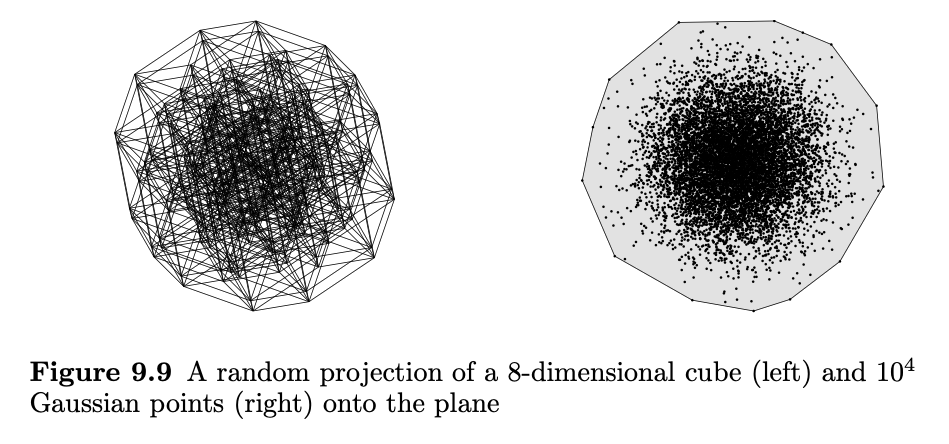
\includegraphics[width=0.8\textwidth]{Chapter 9/fig9-9.png}
\end{center}

It's easier to work with Gaussian projections, where the result says:
\begin{theorem}[Dvoretzky-Milman theorem]
\label{thm:9.7.2}
Let $A$ be an $m \times n$ Gaussian random matrix with i.i.d. $N(0, 1)$ entries, and $T \subset \mathbb{R}^n$ be 
a bounded subset. Then the following holds with probability at least 0.99:
\[ r_- B_2^m \subset \mathrm{conv}(AT) \subset r_+ B_2^m \]
where $B_2^m$ denotes the unit Euclidean ball in $\mathbb{R}^m$, and 
\[ r_{\pm} = w(T) \pm C \sqrt{m} \mathrm{rad}(T). \]
The left inclusion holds only if $r_-$ is nonnegative; the right inclusion always holds.
\end{theorem}

\begin{proof}
Let's use the two-sided Chevet's inequality (\cref{thm:9.7.1}) in the following form:
\[ \mathbb{E}\left[ \sup_{y \in S} \left| \sup_{x \in T}\left\langle Ax, y \right\rangle - w(T) \lVert y 
\rVert_{2} \right| \right] \leq C \gamma(S) \mathrm{rad}(T), \]
where $T \subset \mathbb{R}^n$ and $S \subset \mathbb{R}^m$. To get this, just apply the theorem to $A^T$ with 
$T$ and $S$ swapped.

Let $S$ be the sphere $S^{m - 1}$; its Gaussian complexity satisfies $\gamma(T) \leq \sqrt{m}$. Then, by 
Markov's inequality, the following holds with probability at least 0.99:
\[ \left| \sup_{x \in T}\left\langle Ax, y \right\rangle - w(T) \right| \leq C \sqrt{m} \mathrm{rad}(T) 
\text{ for every } y \in S^{m -1}. \]
By the triangle inequality and the definition of $r_{\pm}$, this implies 
\[ r_- \leq \sup_{x \in T}\left\langle Ax, y \right\rangle \leq r_+ \text{ for every } y \in S^{m - 1}. \]
Rewriting $\sup_{x \in T}\left\langle Ax, y \right\rangle$ as $\sup_{x \in AT}\left\langle x, y \right\rangle$ 
and using homogeneity, we get 
\[ r_- \lVert y \rVert_{2} \leq \sup_{x \in AT}\left\langle x, y \right\rangle \leq r_+ \text{ for every } 
y \in \mathbb{R}^m. \]
By duality (Exercise 9.40), this is the same as the statement of the theorem, and we're done!
\end{proof}

\begin{remark}[The effective dimension]
\label{rmk:9.7.3}
Assume that $T$ is bounded, convex, and contains the origin, and let 
\[ m \leq c d(T) \]
where $d(T) \asymp w(T)^2 / \mathrm{rad}(T)^2$ is the effective dimension (\cref{def:7.5.12}). If we pick the 
absolute constant $c$ to be small enough, we can make $C \sqrt{m} \mathrm{rad}(T) \leq 0.01 w(T)$, so that 
the Dvoretzky-Milman theorem (\cref{thm:9.7.2}) gives
\[ 0.99B \subset AT \subset 1.01B \]
with $B = w(T) B_2^n$ is the Euclidean ball of radius $w(T)$. In short: projecting \textit{any} bounded convex 
set $T$ onto a random subspace of dimension about $d(T)$ makes it look almost like a round ball!
\end{remark}

\begin{example}[Almost round projections of the cube]
\label{ex:9.7.4}
Consider the cube $T = [-1, 1]^n$. By \cref{ex:7.5.7}, 
\[ w(T) = \sqrt{2/\pi} \cdot n \text{ and } \mathrm{diam}(T) = 2 \sqrt{n} \]
So the effective dimension is $d(T) \asymp n$. So, if $m \leq cn$, then with high probability we have 
\[ 0.99B \subset A[-1, 1]^n \subset 1.01B \]
where $B$ is the Euclidean ball with radius $\sqrt{2/\pi} \cdot n$. In short: projecting an $n$-dimensional cube 
onto a subspace of dimension $m = cn$ makes it look almost like a round ball! Figure 9.9 gives an illustration.
\end{example}

\begin{remark}[Summary of random projections]
\label{rmk:9.7.5}
In sections 7.6 and 9.2.2, we found that a random projection $P$ of a set $T$ onto an $m$-dimensional subspace 
in $\mathbb{R}^n$ undergoes a phase transition. In the high-dimensional regime $(m \gtrsim d(T))$, the 
projection shrinks the diameter of $T$ by the factor of order $\sqrt{m/n}$: 
\[ \mathrm{diam}(PT) \asymp \sqrt{\frac{m}{n}} \mathrm{diam}(T)  \]
Moreover, the additive Johnson-Lindenstrauss lemma shows that in this regime, the random projection $P$ 
approximately preserves the geometry of $T$ (the distances between all points in $T$ shrink roughly by the same 
scaling factor).

In the low-dimensional regime $(m \lesssim d(T))$, shrinking stops:
\[ \mathrm{diam}(PT) \asymp w_s(T) \asymp \frac{w(T)}{\sqrt{n}} \]
regardless of how small $m$ is. The Dvoretzky-Milman theorem explains why: $PT$ is now an \textit{approximate 
round ball} of radius of order $w_s(T)$ (Exercise 9.43), which obviously does not shrink under any projection!
\end{remark}


